\usetikzlibrary{backgrounds}

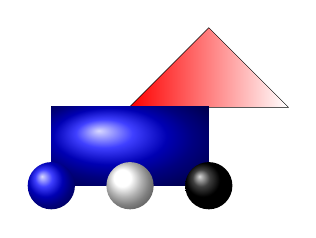
\begin{tikzpicture}

\path[shade,draw] (1,1) -- (2,2)--(3,1)--cycle;
\shade[left color=red] (1,1)--(2,2)--(3,1)--cycle;
\shade[top color=red, bottom color=green](0,0) rectangle (2,1);
\shade[draw,shading=radial, inner color=blue](0,0) rectangle (2,1);
\shade[shading=ball, ball color=blue](0,0) rectangle (2,1);


\shade[shading=ball, ball color=blue] (0,0) circle (.3);
\shade[shading=ball, ball color=white] (1,0) circle (.3);
\shade[shading=ball, ball color=black] (2,0) circle (.3);

\end{tikzpicture}